%
% This work is licensed under a Creative Commons Attribution-ShareAlike 4.0 International License.
% http://creativecommons.org/licenses/by-sa/4.0/
%

% DO NOT COMPILE THIS FILE DIRECTLY!
% This is included by the other .tex files.


\begin{frame}
    
\includegraphics[scale=0.3]{images/logo-circl-Forensics.png}
    \begin{itemize}
        \item[]
        \item[]
        \item[] 3. Disk Acquisition
    \end{itemize}
\end{frame}


\begin{frame}[fragile]
  \frametitle{3.1 Storage devices / media}
    \begin{itemize}
        \item IBM 305 RAMAC - IBM 350 Disk Storage
        \begin{itemize}
            \item 1956: Random Access Method of Accounting and Control
            \item 152 x 172 x 63 cm; 500 kg
            \item 50.000 blocks of 100 Characters $\to$ 5MB
        \end{itemize}
    \end{itemize}
    \begin{figure}
        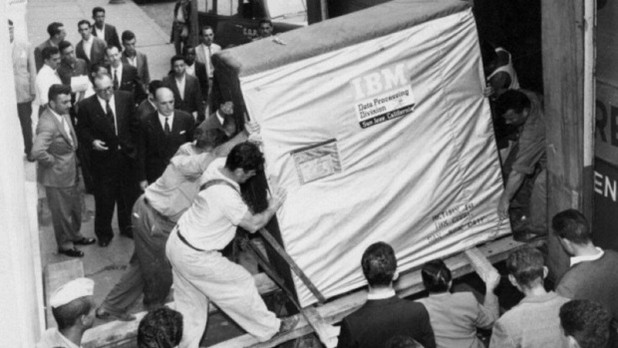
\includegraphics[scale=0.4, angle=0, trim=0 0 0 0]{images/IBM_305.jpeg}
        \captionsetup{labelformat=empty,labelsep=none}
        \transparent{0.4}%
        \caption[]{\tiny Image (c) www.chip.de - Image used solely for illustration purposes}
    \end{figure}
\end{frame}


\begin{frame}[fragile]
  \frametitle{3.1 Storage devices / media}
	\url{ftp://ftp.seagate.com/techsuppt/misc/jet.txt}
  \begin{lstlisting}[basicstyle=\tiny]
 The incredible feat of a read/write head:  Today's new generation of disc
 drives achieve the engineering equivalent of a Boeing 747 flying at MACH 4
 just two meters above the ground, counting each blade of grass as it flies
 over.  The read/write head floats at 12 millionths of an inch above the
 surface of the disc which is turning at 3,600 revolutions per minute.
 Read/write heads position precisely over information tracks which are 800
 millionths of an inch apart and the data is electronically recorded at
 20,000 bits per inch.



                                          __.
                                         / /   - - --
                                       /  /e
                                    ./   /e         /--u O O OO
                              /oAAAAAAAAAAAAAAAAAAA/ 
                            {  @@@  ooooooooooooooo @@'
                              \AAAAAA\AAAA\AAAAAAAAAA/
                                      ue\   \
                                         e\  \
                                            \_\. = = ==

AAAAAAAAAAAAAAAAAAAAAAAAAAAAAAAAAAAAAAAAAAAAAAAAAAAAAAAAAAAAAAAAAAAAA
  \end{lstlisting}
\end{frame}


\begin{frame}[fragile]
  \frametitle{3.1 Storage devices / media}
    \begin{itemize}
        \item Magnetic storage
        \begin{itemize}
            \item Tapes
            \item Floppy disks
            \begin{itemize}
                \item 8" - 1971 - 80KB
                \item 5.25" - 1976 - 360 KB
                \item 3.5" - 1984 - 1.2 MB / - 1986 - 1.44 MB
            \end{itemize}
            \item Hard disks
            \begin{itemize}
                \item IDE / EIDE, Firewire, PATA, SCSI
                \item SATA, SAS Serial attached SCSI, USB, Thunderbolt
            \end{itemize}
        \end{itemize}
        \item Optical storage
        \begin{itemize}
            \item Compact disks - CD
            \item Digital versatile disk - DVD
            \item Blu-ray disk
        \end{itemize}
        \item Non-volatile memory
        \begin{itemize}
            \item USB flash drive
            \item Solid state drive
            \item Flash memory cards
        \end{itemize}
    \end{itemize}
\end{frame}


\begin{frame}[fragile]
  \frametitle{3.2 Physical- / Logical layers}
  \begin{lstlisting}[basicstyle=\tiny]
	       Mass storage device
 ---------    ---------    ---------    ---------     Considerations: Disk duplication
| 8 TByte |  | 8 TByte |  | 8 TByte |  | 8 TByte |
 ---------    ---------    ---------    ---------         Speed USB2: 480 Mbit/s
     |            |            |            |               Capacity: 8 * 1024^4 * 8
     V            V            V            V               Duration: ~40 hours per disk
     RAID
   --------------------------------------------
  |  System  Data                              |        Speed USB3.1: 10 Gbit/s
  |  ----------------------------------------  |            Capacity: 24 * 1024^4 * 8
  | |  P1  |    P2 (24 TByte)                | |            Duration: ~5 hours per volume
  |  ----------------------------------------  |
   --------------------------------------------             (Theoretically)


A solution:
	- Local NAS
	- 10 GBit network
	- USB 3.1 / 3.2
	- 60+ TB mass storage
	- Virtual appliance
  \end{lstlisting}
\end{frame}


\begin{frame}[fragile]
  \frametitle{3.3 ATA Disks }
    \begin{itemize}
        \item ATA-3: Hard disk password
        \item ATA-4: HPA - Host Protected Area
        \begin{itemize}
            \item Vendor area - benefit system vendors
            \item Recovery data. persistent data
            \item Controlled by firmware not OS
            \item \texttt{READ\_NATIVE\_MAX\_ADDRESS}
        \end{itemize}
        \item ATA-6: DCO - Device Configuration Overlay
        \begin{itemize}
            \item Benefit system vendors
            \item Control reported capacity and disk features
            \item Use disk from different manufacturers
            \item Use disk with different number of sectors
            \item[] $\to$ Makes disks looking uniq
            \item \texttt{DEVICE\_CONFIGURATION\_IDENTIFY}
        \end{itemize}
        \item ATA-7: Serial ATA
    \end{itemize}
\end{frame}


\begin{frame}[fragile]
  \frametitle{3.4 Demo: Hidden Sectors}
    \begin{itemize}
        \item New disk
\begin{lstlisting}[basicstyle=\tiny]
dmesg
    sd 1:0:0:0: [sdb] 3904981168 512-byte logical blocks: (2.00 TB/1.82 TiB)

hdparm -N /dev/sdb
    max sectors   = 3907029168/3907029168, ACCESSIBLE MAX ADDRESS disabled
\end{lstlisting}
        \item Create hidden message
\begin{lstlisting}[basicstyle=\tiny]
echo -n 'MySecret 123456' | dd of=/dev/sdb seek=3500000000

dd if=/bin/dd of=/dev/sdb seek=3500000001
     148+1 records in
     148+1 records out
     76000 bytes (76 kB, 74 KiB) copied, 0,022659 s, 3,4 MB/s
\end{lstlisting}
        \item Create HPA
\begin{lstlisting}[basicstyle=\tiny]
hdparm --yes-i-know-what-i-am-doing -N p3000000000 /dev/sdb
    setting max visible sectors to 3000000000 (permanent)
    max sectors   = 3000000000/3907029168, ACCESSIBLE MAX ADDRESS enabled

Power cycle your device after every ACCESSIBLE MAX ADDRESS
\end{lstlisting}
    \end{itemize}
\end{frame}


\begin{frame}[fragile]
  \frametitle{3.4 Demo: Hidden Sectors}
    \begin{itemize}
        \item Create partition and format
\begin{lstlisting}[basicstyle=\tiny]
dmesg
    sd 1:0:0:0: [sdb] 3000000000 512-byte logical blocks: (1.54 TB/1.40 TiB)

fdisk /dev/sdb
    primary
    2048
    2999999999

mkfs.ntfs -L CIRCL.DFIR -f /dev/sdb1
    Creating NTFS volume structures.
    mkntfs completed successfully. Have a nice day.
\end{lstlisting}
        \item Investigate disk layout
\begin{lstlisting}[basicstyle=\tiny]
fdisk -l /dev/sdb
    Device     Boot Start        End    Sectors  Size Id Type
    /dev/sdb1        2048 2999999999 2999997952  1,4T  7 HPFS/NTFS/exFAT
\end{lstlisting}
        \item Investigate last accessible sector
\begin{lstlisting}[basicstyle=\tiny]
dd if=/dev/sdb skip=2999999999 status=none| xxd
    00000000: eb52 904e 5446 5320 2020 2000 0208 0000  .R.NTFS    .....
      .......
    000001f0: 0000 0000 0000 0000 0000 0000 0000 55aa  ..............U.
\end{lstlisting}
    \end{itemize}
\end{frame}


\begin{frame}[fragile]
  \frametitle{3.4 Demo: Hidden Sectors}
    \begin{itemize}
        \item Try to access hidden message
\begin{lstlisting}[basicstyle=\tiny]
dd if=/dev/sdb skip=3500000000 count=1 | xxd
    dd: /dev/sdb: cannot skip: Invalid argument
    0+0 records in
\end{lstlisting}
        \item Resize HPA
\begin{lstlisting}[basicstyle=\tiny]
hdparm -N /dev/sdb
    max sectors   = 3000000000/3907029168, ACCESSIBLE MAX ADDRESS enabled

hdparm --yes-i-know-what-i-am-doing -N p3900000000 /dev/sdb
    max sectors   = 3900000000/3907029168, ACCESSIBLE MAX ADDRESS enabled

Power cycle your device after every ACCESSIBLE MAX ADDRESS
\end{lstlisting}
        \item Investigate disk layout and last sector
\begin{lstlisting}[basicstyle=\tiny]
fdisk -l /dev/sdb
    Device     Boot Start        End    Sectors  Size Id Type
    /dev/sdb1        2048 2999999999 2999997952  1,4T  7 HPFS/NTFS/exFAT

dd if=/dev/sdb skip=2999999999 status=none | xxd | less
dd if=/dev/sdb skip=3899999999 status=none | xxd | less
\end{lstlisting}
    \end{itemize}
\end{frame}


\begin{frame}[fragile]
  \frametitle{3.4 Demo: Hidden Sectors}
    \begin{itemize}
        \item Recover hidden message
\begin{lstlisting}[basicstyle=\tiny]
dd if=/dev/sdb skip=3500000000 count=1 status=none
    00000000: 4d79 5365 6372 6574 2031 3233 3435 3600  MySecret 123456.
\end{lstlisting}
	\item Recover hidden \texttt{dd} command
\begin{lstlisting}[basicstyle=\tiny]
dd if=/dev/sdb skip=$(( 3500000001*512 )) count=76000 bs=1 of=dd.exe

md5sum dd.exe
    36a70f825b8b71a3d9ba3ac9c5800683

md5sum /bin/dd
    36a70f825b8b71a3d9ba3ac9c5800683
\end{lstlisting}
        \item Feeback: kaplan(at)cert.at
\begin{lstlisting}[basicstyle=\tiny]
    https://www.schneier.com/blog/archives/2014/02/swap_nsa_exploi.html
    https://en.wikipedia.org/wiki/Host_protected_area
\end{lstlisting}
        \item How it works
\begin{lstlisting}[basicstyle=\tiny]
    IDENTIFY DEVICE
    SET MAX ADDRESS
    READ NATIVE MAX ADDRESS
    --> HPA aware software (like the BIOS)
\end{lstlisting}
    \end{itemize}
\end{frame}


\begin{frame}[fragile]
  \frametitle{3.5 Other Hidden Sectors}
    \begin{itemize}
        \item Service area, negative sectors
        \begin{itemize}
            \item Firmware
            \item Bad sectors
            \item ATA passwords
            \item[] \texttt{hdparm --security-unlock "myPassWD" /dev/sdb}
            \item SMART data
	    \item[]
        \end{itemize}
        \item Self-Monitoring, Analysis and Reporting Technology - SMART
        \begin{itemize}
            \item[] \texttt{apt install smartmontools}
            \item[] \texttt{smartctl -x /dev/sdb | less}
\begin{lstlisting}[basicstyle=\tiny]
.....
SMART Attributes Data Structure revision number: 16
Vendor Specific SMART Attributes with Thresholds:
ID# ATTRIBUTE_NAME          FLAGS    VALUE WORST THRESH FAIL RAW_VALUE
  1 Raw_Read_Error_Rate     POSR-K   200   200   051    -    0
  3 Spin_Up_Time            POS--K   234   233   021    -    3258
  4 Start_Stop_Count        -O--CK   100   100   000    -    679
  5 Reallocated_Sector_Ct   PO--CK   200   200   140    -    0
  7 Seek_Error_Rate         -OSR-K   200   200   000    -    0
  9 Power_On_Hours          -O--CK   095   095   000    -    3802
  .....
\end{lstlisting}
        \end{itemize}
    \end{itemize}
\end{frame}


\begin{frame}[fragile]
  \frametitle{3.6 Collecting information from devices}
    \begin{itemize}
        \item[] \texttt{hdparm -I /dev/sdb}
\begin{lstlisting}[basicstyle=\tiny]
ATA device, with non-removable media
        Model Number:       WDC WD20NPVT-00Z2TT0                    
        Serial Number:      WD-WX11A9269540
        Firmware Revision:  01.01A01
        Transport:          Serial, SATA 1.0a, SATA Rev 2.6, SATA Rev 3.0
Standards:
        Supported: 8 7 6 5 
        Likely used: 8
	.....
Security: 
        Master password revision code = 65534    supported
        not     enabled
        not     locked
        not     frozen
        not     expired: security count
        374min for SECURITY ERASE UNIT.
\end{lstlisting}
        \item[] \texttt{hdparm -I /dev/sda}
\begin{lstlisting}[basicstyle=\tiny]
...
Commands/features:
        Enabled Supported:
        ...
           *    Data Set Management TRIM supported (limit 8 blocks)
           *    Deterministic read ZEROs after TRIM
\end{lstlisting}
    \end{itemize}
\end{frame}














\begin{frame}[fragile]
  \frametitle{3.7 How is the device connected}
    \begin{itemize}
        \item Most relevant data with: \texttt{dmesg}
\begin{lstlisting}[basicstyle=\tiny]
dmesg -T
    .....
    [Mi Aug  1 13:06:11 2018] usb-storage 1-1:1.0: USB Mass Storage device detected
    [Mi Aug  1 13:06:11 2018] scsi host1: usb-storage 1-1:1.0
    [Mi Aug  1 13:06:13 2018] scsi 1:0:0:0: Direct-Access USB Flash DISK
    [Mi Aug  1 13:06:13 2018] sd 1:0:0:0: Attached scsi generic sg1 type 0
    [Mi Aug  1 13:06:13 2018] sd 1:0:0:0: [sdb] 15826944 512-byte logical blocks
\end{lstlisting}
        \item Enumerate host hardware
\begin{lstlisting}[basicstyle=\tiny]
lshw | less
    .....

lshw -businfo -class storage
    Bus info          Device           Class          Description
    =============================================================
    pci@0000:04:00.0                   storage        Samsung Electronics Co Ltd
    usb@2:3           scsi0            storage        
    usb@1:1           scsi1            storage

lshw -businfo -class disk
    Bus info          Device           Class          Description
    =============================================================
    scsi@0:0.0.0      /dev/sda         disk           SD/MMC CRW
                      /dev/sda         disk
    scsi@1:0.0.0      /dev/sdb         disk           2TB 2000FYYZ-01UL1B2
\end{lstlisting}
    \end{itemize}
\end{frame}


\begin{frame}[fragile]
  \frametitle{3.7 How is the device connected}
    \begin{itemize}
        \item Enumerate PCI bus
\begin{lstlisting}[basicstyle=\tiny]
lspci -d ::0106                      # List SATA controller

lspci -d ::0108                      # List NVME controller
    04:00.0 Non-Volatile memory controller: Samsung Electronics Co Ltd Device a808

lspci -d ::0C03                      # List USB, FW, ... controller
    00:14.0 USB controller: Intel Corporation Sunrise Point-LP USB 3.0 xHCI Controller (rev 21)
    3b:00.0 USB controller: Intel Corporation JHL6540 Thunderbolt 3 USB Controller (C step) [Alpine Ridge 4C 2016] (rev 02)
    3e:00.0 USB controller: Fresco Logic FL1100 USB 3.0 Host Controller (rev 10)
    40:00.0 USB controller: Fresco Logic FL1100 USB 3.0 Host Controller (rev 10)
\end{lstlisting}
        \item Enumerate block devices
\begin{lstlisting}[basicstyle=\tiny]
lsscsi -v

lsblk /dev/sdb
    NAME   MAJ:MIN RM  SIZE RO TYPE MOUNTPOINT
    sdb      8:16   0  1,8T  0 disk
     sdb1   8:17   0  1,8T  0 part /media/mich/031F0F30642CBB8B

lsblk -pd -o TRAN,NAME,SERIAL,VENDOR,MODEL,REV,WWN,SIZE,HCTL,SUBSYSTEMS /dev/sdb
    TRAN NAME     SERIAL          VENDOR   MODEL
    usb  /dev/sdb WD-WMC1P0H10ZEX WT055 WD 2000FYYZ-01UL1B2
             REV WWN                 SIZE HCTL       SUBSYSTEMS
            01.0 0x50014ee05979e023  1,8T 1:0:0:0    block:scsi:usb:pci
\end{lstlisting}
    \end{itemize}
\end{frame}


\begin{frame}[fragile]
	\frametitle{3.8 USB enumeration}
    \begin{itemize}
        \item List attached USB device
        \begin{itemize}
            \item USB bus
            \item Device address
            \item Vendor ID
            \item Product ID
            \item Product details
            \item[] ...
        \end{itemize}
        \item[] \texttt{lsusb}
\begin{lstlisting}[basicstyle=\tiny]
Bus 004 Device 001: ID 1d6b:0003 Linux Foundation 3.0 root hub
Bus 003 Device 001: ID 1d6b:0002 Linux Foundation 2.0 root hub
Bus 002 Device 002: ID 0bda:0328 Realtek Semiconductor Corp. 
Bus 002 Device 003: ID 1b1c:1a0e Corsair 
Bus 002 Device 004: ID 0951:162b Kingston Technology 
Bus 002 Device 001: ID 1d6b:0003 Linux Foundation 3.0 root hub
Bus 001 Device 004: ID 06cb:009a Synaptics, Inc. 
Bus 001 Device 003: ID 04f2:b61e Chicony Electronics Co., Ltd 
Bus 001 Device 001: ID 1d6b:0002 Linux Foundation 2.0 root hub
\end{lstlisting}
    \end{itemize}
\end{frame}


\begin{frame}[fragile]
	\frametitle{3.8 USB enumeration}
    \begin{itemize}
        \item[] \texttt{lsusb -t}
\begin{lstlisting}[basicstyle=\tiny]
/:  Bus 04.Port 1: Dev 1, Class=root_hub, Driver=xhci_hcd/2p, 10000M
/:  Bus 03.Port 1: Dev 1, Class=root_hub, Driver=xhci_hcd/2p, 480M
/:  Bus 02.Port 1: Dev 1, Class=root_hub, Driver=xhci_hcd/6p, 5000M
    |__ Port 1: Dev 4, If 0, Class=Mass Storage, Driver=usb-storage, 5000M
    |__ Port 2: Dev 3, If 0, Class=Mass Storage, Driver=uas, 5000M
    |__ Port 3: Dev 2, If 0, Class=Mass Storage, Driver=usb-storage, 5000M
/:  Bus 01.Port 1: Dev 1, Class=root_hub, Driver=xhci_hcd/12p, 480M
    |__ Port 8: Dev 3, If 1, Class=Video, Driver=uvcvideo, 480M
    |__ Port 8: Dev 3, If 0, Class=Video, Driver=uvcvideo, 480M
    |__ Port 9: Dev 4, If 0, Class=Vendor Specific Class, Driver=, 12M
\end{lstlisting}
        \item[] \texttt{lsusb  -v -d 0951:162b`}
\begin{lstlisting}[basicstyle=\tiny]
...
    Interface Descriptor:
      bLength                 9
      bDescriptorType         4
      bInterfaceNumber        0
      bAlternateSetting       0
      bNumEndpoints           2
      bInterfaceClass         8 Mass Storage
      bInterfaceSubClass      6 SCSI
      bInterfaceProtocol     80 Bulk-Only
...
\end{lstlisting}
    \end{itemize}
\end{frame}


\begin{frame}[fragile]
    \frametitle{3. usbmon \& wireshark}
	\frametitle{3.9 USB Interface monitoring}
    \begin{figure}
        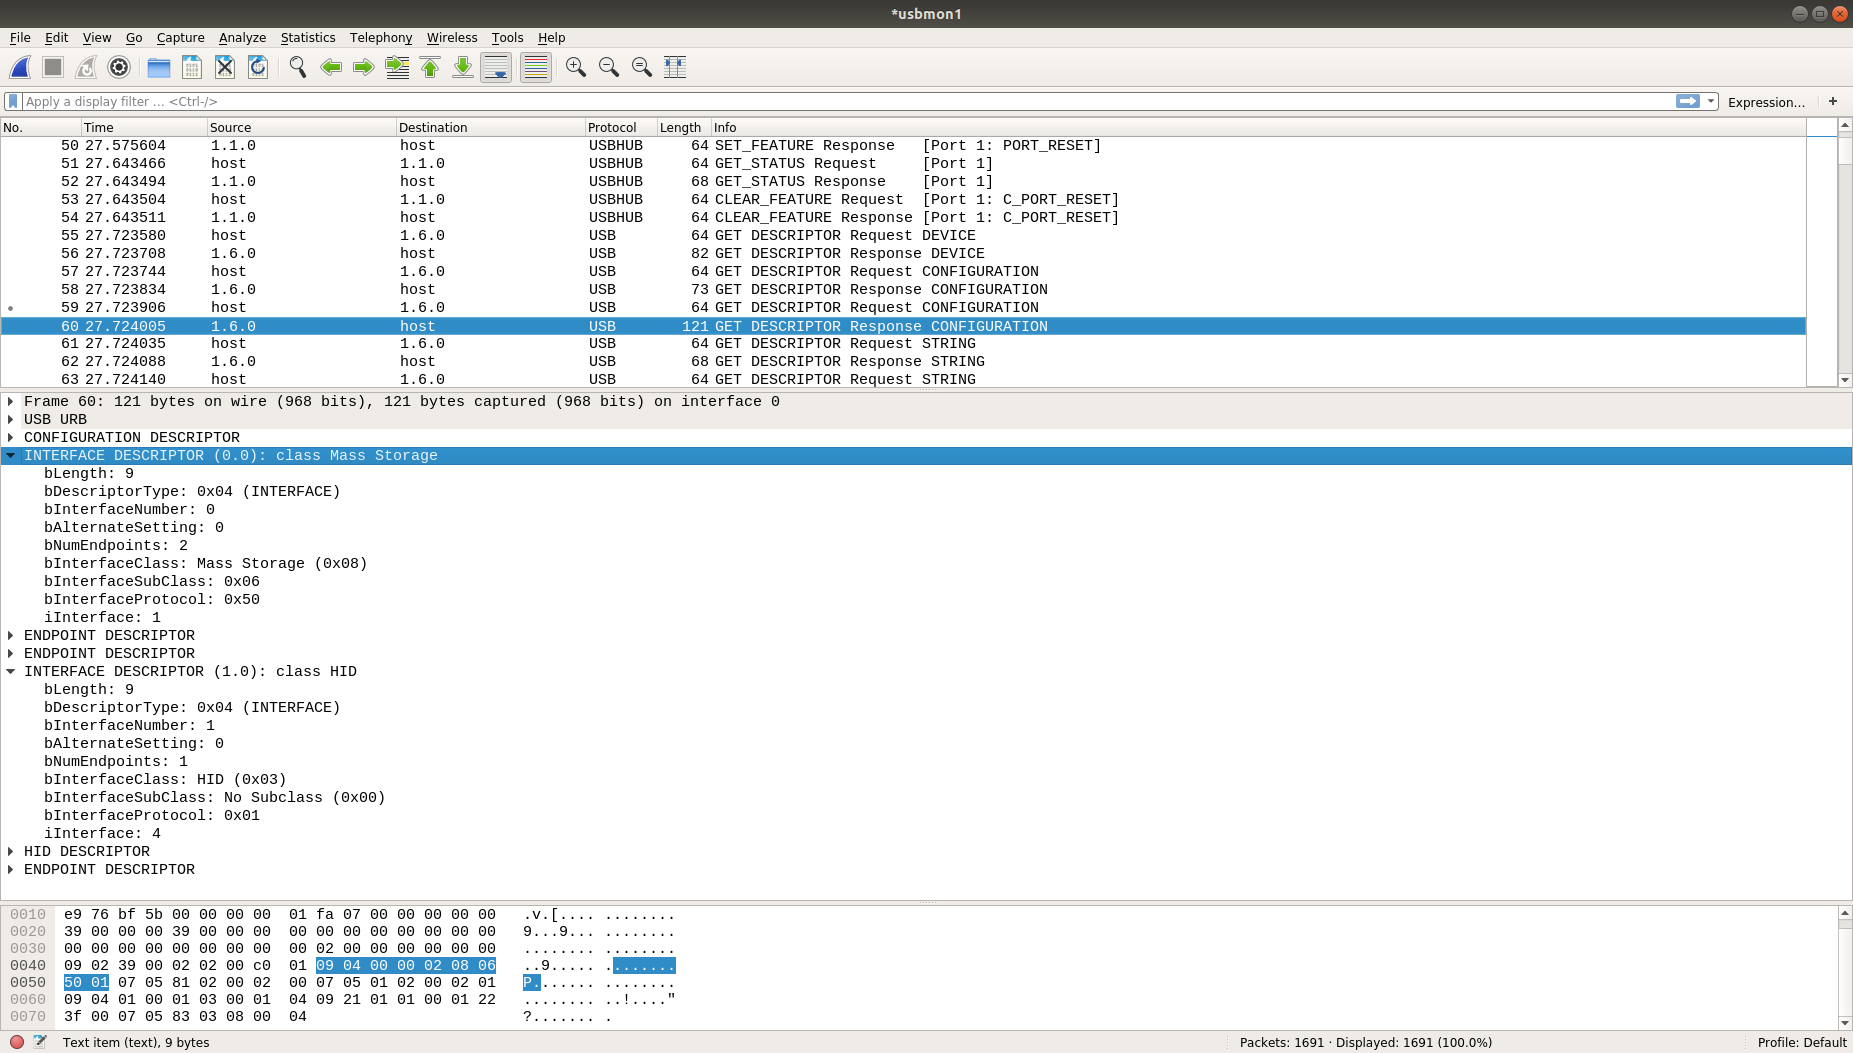
\includegraphics[scale=0.18, angle=0, trim=0 0 0 0]{images/usbmon.png}\llap{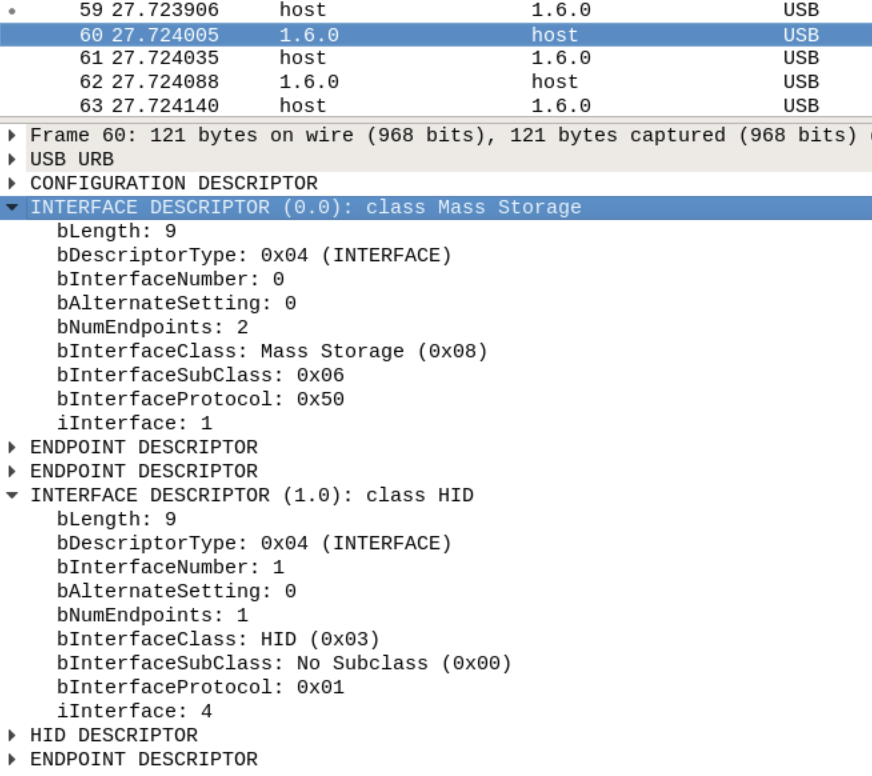
\includegraphics[scale=0.27, trim = 0px 0px 0px 0px, angle=-5]{images/usbmon2.png}}
        % 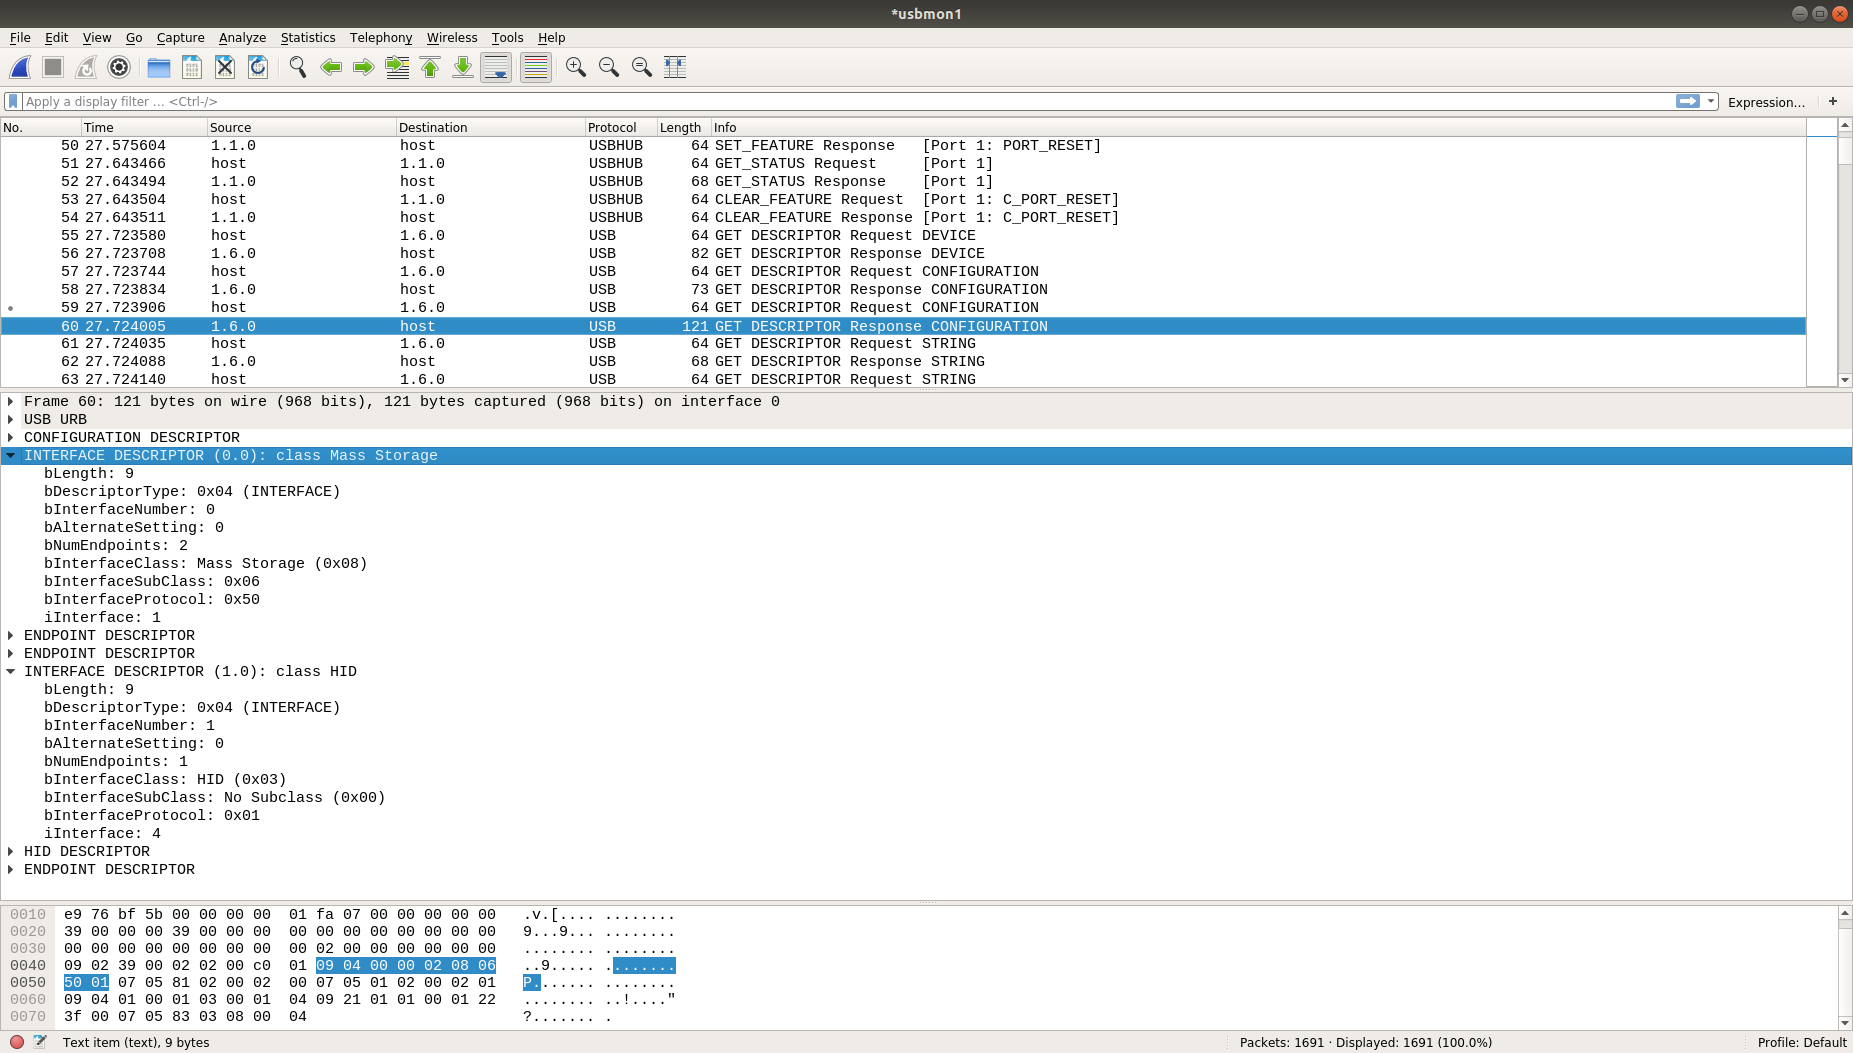
\includegraphics[scale=0.18, angle=0, trim=0 0 0 0]{images/usbmon.png}\llap{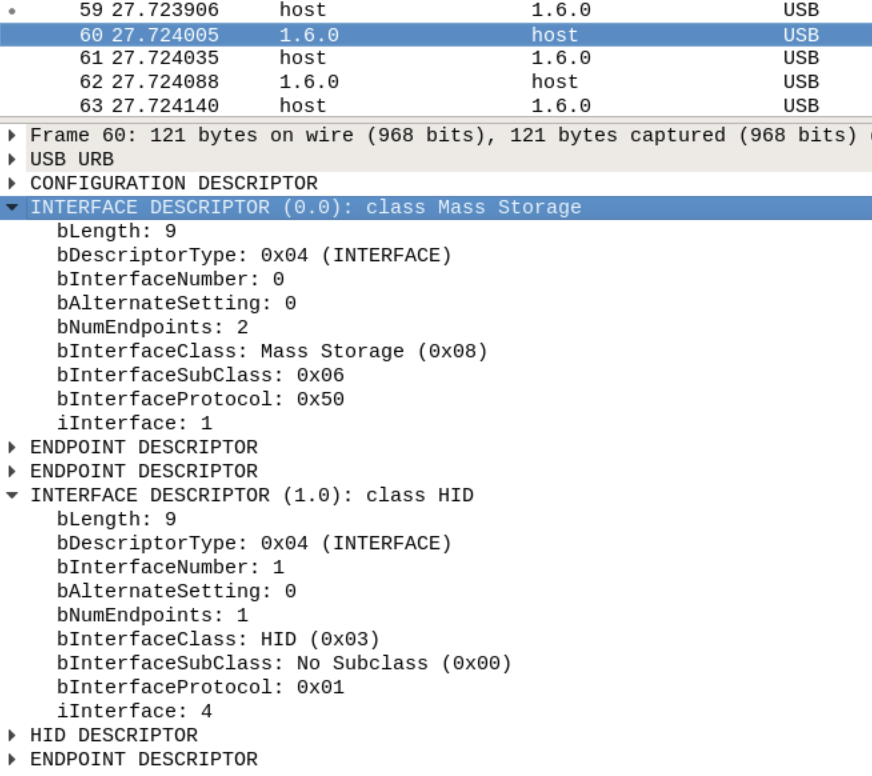
\includegraphics[height=5cm]{images/usbmon2.png}}
        \captionsetup{labelformat=empty,labelsep=none}
    \end{figure}
\end{frame}



